\chapter{\ifproject%
\ifcpe โครงสร้างและขั้นตอนการทำงาน\else Project Structure and Methodology\fi
\else%
\ifcpe โครงสร้างของโครงงาน\else Project Structure\fi
\fi
}

% ในบทนี้จะกล่าวถึงหลักการ และการออกแบบระบบ

\makeatletter

% \renewcommand\section{\@startsection {section}{1}{\z@}%
%                                    {13.5ex \@plus -1ex \@minus -.2ex}%
%                                    {2.3ex \@plus.2ex}%
%                                    {\normalfont\large\bfseries}}

\makeatother
%\vspace{2ex}
% \titleformat{\section}{\normalfont\bfseries}{\thesection}{1em}{}
% \titlespacing*{\section}{0pt}{10ex}{0pt}

\section{Model View Controller (MVC)}
โครงงานนี้ใช้ design pattern MVC~\cite{mvc}\CIreply{ทำไมเป็นคำว่า ``และ''}แบ่งออกเป็น 3 ส่วนหลักๆ ดังรูปที่ \ref{mvc} คือ 
\begin{enumerate}
    \item Model
    \item View
    \item Controller
\end{enumerate}

\begin{figure}
\begin{center}
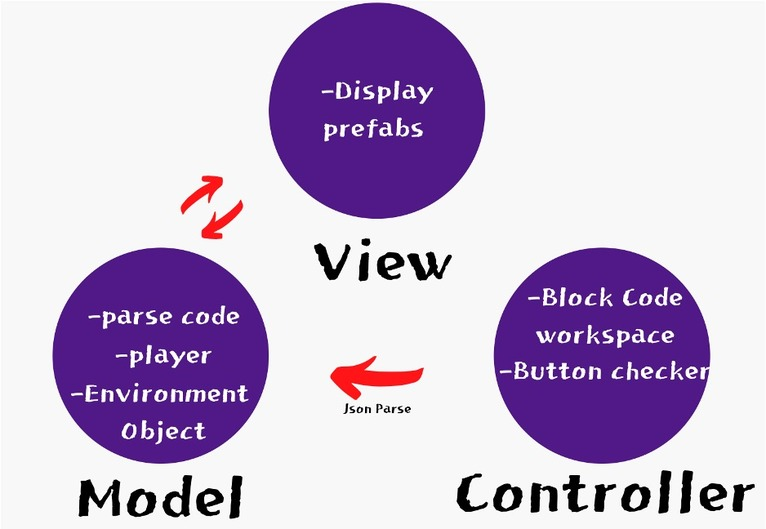
\includegraphics{pic/pic1.jpg}
\end{center}
\caption[Poem]{Design Pattern MVC}
\label{mvc}
\end{figure}

\subsection{Model}
 ในส่วนของ Model จะเป็นการจัดการแปลงจาก Block Code ให้เป็น C\# เพื่อทำให้เกิด Event ต่างๆ เช่นการเดิน, การหมุน
 และการกระโดด เป็นต้น โดยที่ Model จะรับBlock Code มาจาก Controller ในรูปของ JSON
 และจะทำการแปลงเป็น C\# เพื่อสั่งให้ view แสดงผลต่างๆ ส่วนของ Model จะอยู่ใน Unity
 เป็นตัวกลางในการสื่อสารระหว่าง View กับ Controller

\subsection{View}
View นั้นทำหน้าที่แค่แสดงผลโดยรับโค้ดคำสั่งมาจาก Model และทำการแสดงผล จากนั้นจะทำการ
ส่งค่าคืน เพื่อบอก Model ว่าแสดงผลตามตามคำสั่งนั้นแล้ว ในส่วนของ View นั้นจะอยู่ใน
Unity เช่นกัน เพราะ View ใช้แสดงผลกราฟฟิกของ Unity ที่ผู้พัฒนาได้สร้างเอาไว้ เช่น prefabs(รูปแบบสำเร็จ) ต่างๆ ดังรูปที่ \ref{prefabs}
รวมไปถึงการแสดงหน้า UI ของเกม ซึ่งจะกล่าวถึงในหัวข้อ User Interface\par

\begin{figure}
    \begin{center}
    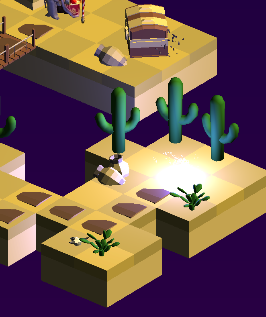
\includegraphics{pic/prefap.PNG}
    \end{center}
    \caption[Poem]{ตัวอย่าง prefabs ที่ใช้ }
    \label{prefabs}
    \end{figure}
    


\subsection{Controller}
Controller จะอยู่ทั้ง 2 ฝั่ง คือทั้ง Unity และ WebView โดย Controller ฝั่งหน้าเว็ปจะเป็นการรอให้ผู้ใช้
ลากวางตัว Block Code และเมื่อผู้ใช้กดรัน Controller ฝั่งหน้าเว็ปจะทำการแปลง Block Code ให้เป็น Object 
ในรูปของ JSON และจะถูกนำส่งไปให้ Controller ฝั่ง Unity หลักจากนั้น Controller ฝั่ง Unity จะทำการ
ประมวลผลและแปลงเป็น Object ที่ Unity สามารถอ่านได้เพื่อส่งต่อไปให้ Model

\section{User Interface (UI)}
User interface (UI) คือ การออกแบบที่เน้นไปที่เรื่องหน้าตา ความสวยงาม และทุกอย่างที่จะเป็นการโต้ตอบกับผู้ใช้งาน UI ที่ดีจะช่วยดึงดูดผู้ใช้งานให้เกิดความสนใจและช่วยให้ผู้ใช้งานเข้าถึงข้อมูลได้ง่าย
โดยการออกแบบ UI ของเกมนี้พวกเราจะออกแบบเกมแนวตะลุยอวกาศ โดยจะใช้ Asset ที่มีอยู่ใน Unity มาปรับแต่งจัดวางเพื่อความสวยงามและความน่าสนใจ โดยจะมีส่วนต่างๆ ดังนี้ ซึ่งจะแสดงดังรูปต่อไปนี้
\begin{itemize}
\item หน้าจอแสดง Mainmenu รูปที่ \ref{mainmenu}
\item หน้าจอแสดงหน้าเลือกด่าน รูปที่ \ref{stage}
\item หน้าต่างแสดงเมนูการตั้งค่า รูปที่ \ref{setting}
\item หน้าจอแสดงหน้า Gameplay รูปที่ \ref{game}
\item หน้าต่างที่แสดงว่าเราชนะ รูปที่ \ref{win}
\item หน้าต่างที่แสดงว่าเราแพ้ รูปที่ \ref{lose}
\end{itemize}


\begin{figure}
\begin{center}
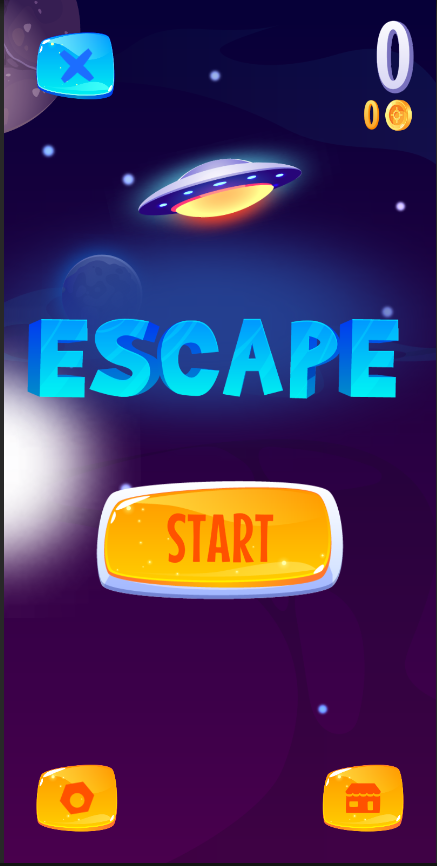
\includegraphics[scale = 0.4]{pic/home_start.PNG}
\end{center}
\caption[Poem]{หน้า Mainmenu ของเกม}
\label{mainmenu}
\end{figure}

\begin{figure}
\begin{center}
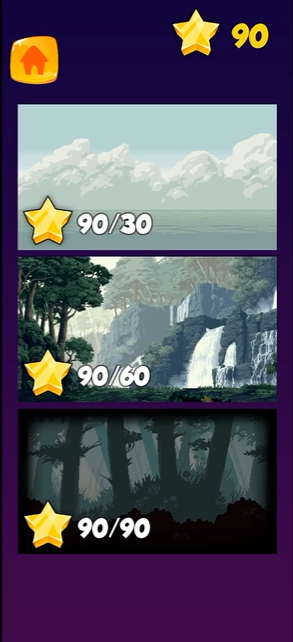
\includegraphics[scale = 0.4]{pic/MapSelection.png}
\end{center}
\caption[Poem]{หน้าเลือกด่าน}
\label{stage}
\end{figure}

\begin{figure}
\begin{center}
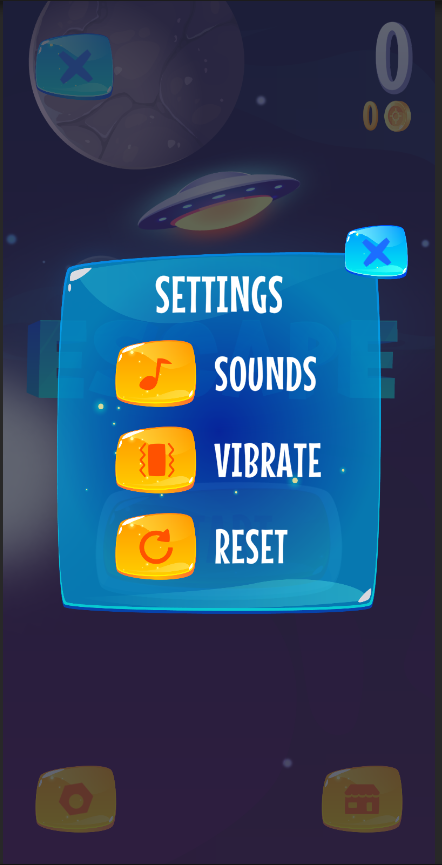
\includegraphics[scale = 0.4]{pic/setting.PNG}
\end{center}
\caption[Poem]{เมนูการตั้งค่า}
\label{setting}
\end{figure}

\begin{figure}
\begin{center}
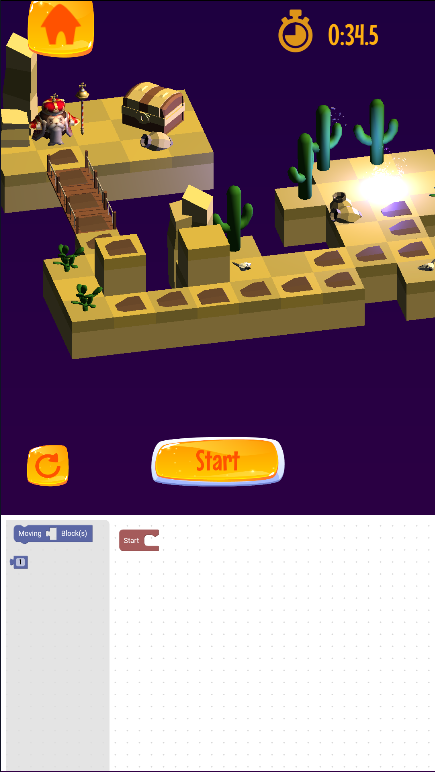
\includegraphics[scale = 0.4]{pic/gameplay.PNG}
\end{center}
\caption[Poem]{หน้า Gameplay}
\label{game}
\end{figure}

\begin{figure}
\begin{center}
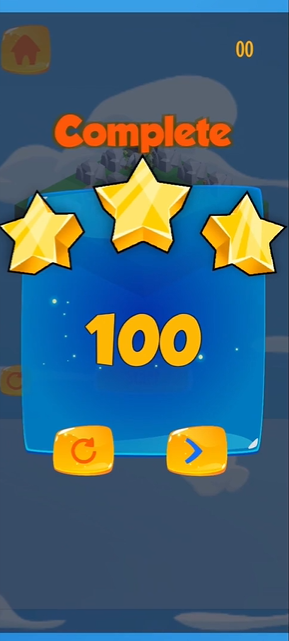
\includegraphics[scale = 0.4]{pic/Complete.png}
\end{center}
\caption[Poem]{หน้าต่างที่แสดงว่าชนะ}
\label{win}
\end{figure}

\begin{figure}
\begin{center}
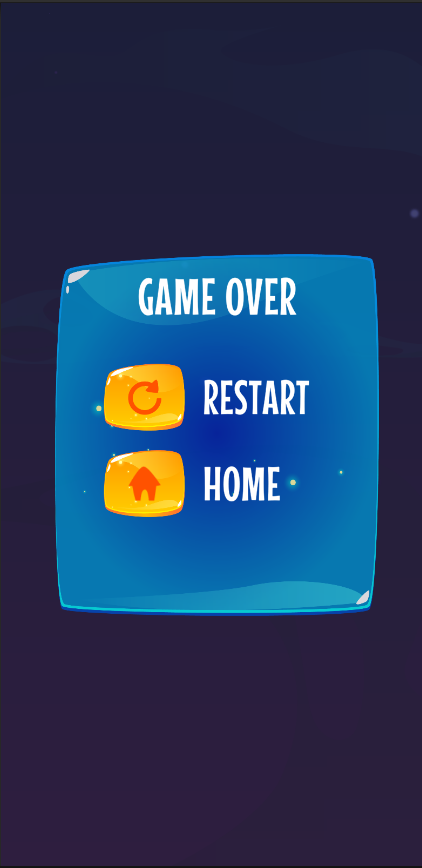
\includegraphics[scale = 0.4]{pic/gameover.PNG}
\end{center}
\caption[Poem]{หน้าต่าง GameOver}
\label{lose}
\end{figure}



\section{WebView}
ตัวหน้าเว็ปทำขึ้นมาเพื่อนำ Google Blockly ไปใส่ใน panel ของ Unity เพราะเดิมที Unity ไม่สามารถสร้าง Object ที่หน้าตาและรวมไปถึง function ที่เหมือนกับ Google Blockly ได้ ทางผู้พัฒนาเลยสร้างหน้าเว็ปเข้ามาเพื่อนำไปใส่ใน 
panel ของ Unity ที่ใช้ในการแสดงผล Block Code


\begin{figure}
\begin{center}
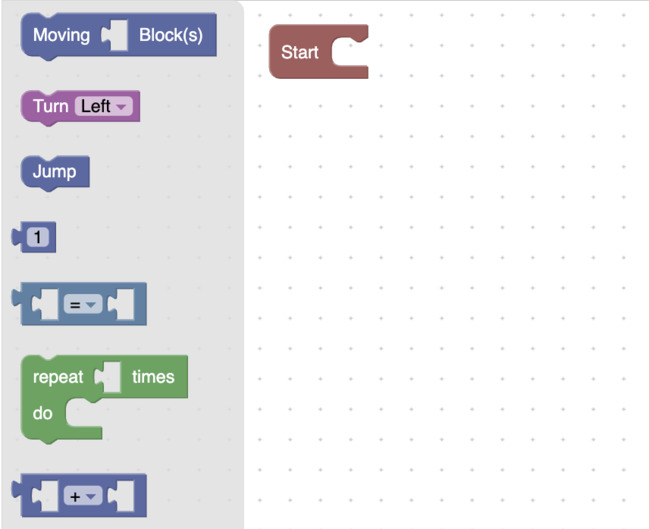
\includegraphics{pic/block1.jpg}
\end{center}
\caption[Poem]{Google Blockly}
\label{block}
\end{figure}

\section{Text Reader}
การสร้างด่านของเกมนี้จะ Input ด้วยไฟล์ Text กล่าวคือเมื่อ User ทำการ Input ไฟล์มาตัวระบบเกมจะทำการจัดการสร้างด่านให้เอง
ทำให้การที่จะสร้างด่านหนึ่งด่านไม่ต้องทานั่งลากวางตัว prefabs บน Unity ตัวอย่างไฟล์ Text คร่าวๆ จากรูป\ref{txt}
\begin{figure}
    \begin{center}
    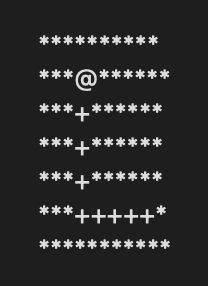
\includegraphics{pic/text.png}
    \end{center}
    \caption[Poem]{Text}
    \label{txt}
    \end{figure}
